\begin{figure}[ht]
	\centering
	\footnotesize

	\psfrag{x}[l][l] {$\theta$}
	\psfrag{t0}[l][l] {$\phi(\theta)$}

	\psfrag{one}[r][r] {$1$}
	\psfrag{half}[r][r] {$0.5$}

	\psfrag{delta}[l][l] {$\phi(\theta) = \delta \theta$}
	\psfrag{md}[l][l] {$\displaystyle \phi(\theta) = \frac{1+\theta}{2}$}
	\psfrag{gma}[l][l] {$\phi(\theta) = \gamma$}

	\psfrag{oh}[l][l] {$O$}

	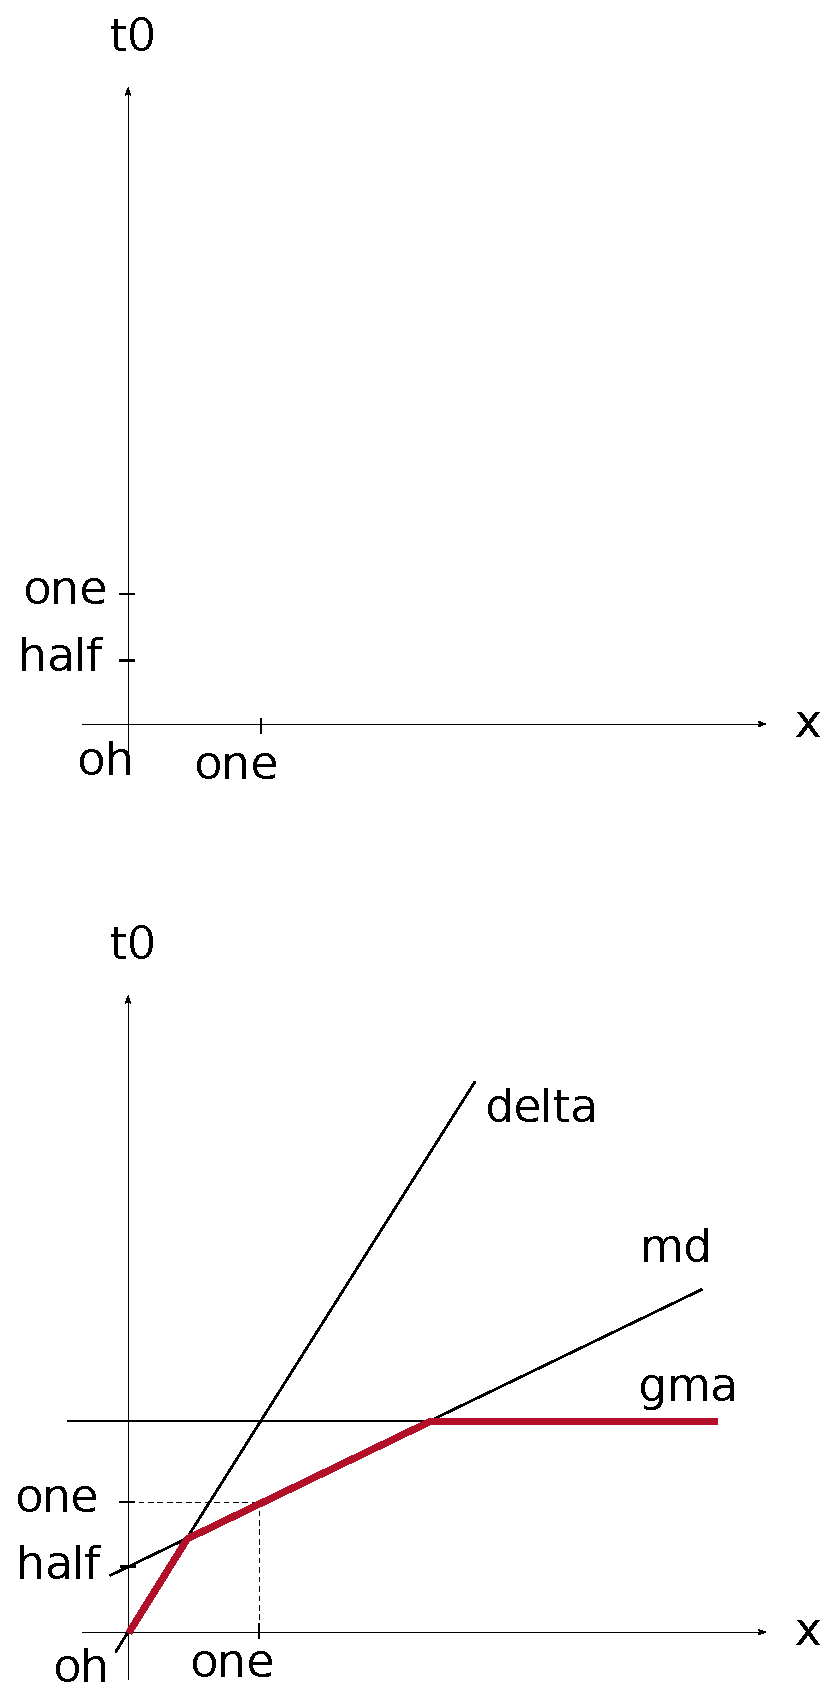
\includegraphics[width=0.55\textwidth]{limiter1.eps}
	\caption{Limiter function
		$\displaystyle \phi(\theta) =
			\min\left(\delta \theta, \frac{1+\theta}{2}, \gamma \right),
			\ \text{for} \ \delta,\gamma \geq 1$.}
	\label{\LABEL}
\end{figure}